\documentclass[10pt]{exam}
\usepackage[hon]{template-for-exam}
\usepackage{tikz,ifthen}
\footer{\emph{\small Example Problems: Ch 3 (Two-Dimensional Motion)}}{}{\sc \myclass}


\title{Chapter 3 Example Problems}
\author{Rohrbach}
\date{\today}

\begin{document}
\maketitle

\def\mystrut{\protect\rule[-2.2ex]{0ex}{2.2ex}} 
\qformat{ \textbf{Example Problem 3-\thequestion}
  \ifthenelse{\equal{\thequestion}{\thequestiontitle}}
    {}
    {: \emph{\thequestiontitle}}
  \mystrut  \hfill}
\begin{questions}
  
\titledquestion{Adding Vectors}
  
  Vectors $\vec{A}$ and $\vec{B}$ are shown below.

  \begin{parts}
    \part 
      Find the components of $\vec{A}$ and $\vec{B}$.
    \part
      Sketch out $\vec{R}=\vec{A}-2\vec{B}$.
    \part
      Calculate the $x$- and $y$- components of $\vec{R}$
    \part
      Calculate the magnitude and direction of $\vec{R}$
  \end{parts}

  \vspace{1em}

  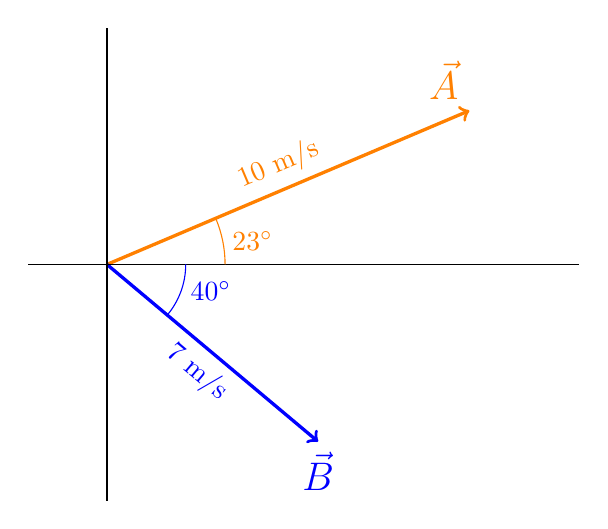
\begin{tikzpicture}[
    vector/.style={
      ->,
      very thick,
    }
  ]
    \def\unit{0.5}
    

    \draw[vector,orange] (0,0) -- (23:10*\unit) 
      node[anchor=south east] {\Large $\vec{A}$} 
      node[midway,above,rotate=23] {10 m/s};
    \draw[vector,blue] (0,0) -- (-40:7*\unit)
      node[anchor=north] {\Large $\vec{B}$}
      node[midway,below,rotate=-40] {7 m/s};
    \draw (0,3) -- (0,-3);
    \draw (-1,0) -- (6,0);

    \draw[orange] (1.5,0) arc (0:23:1.5) 
      node[midway,right] {$23^\circ$};
    \draw[blue] (1,0) arc (0:-40:1) 
      node[midway,right] {$40^\circ$};



  \end{tikzpicture}

\pagebreak

\titledquestion{Projectiles Launched Horizontally}
  A marble rolls off a 0.8-meter tall table at a horizontal speed of 3 m/s.

  \begin{parts}
    \part 
      How far from the base of the table will the marble land?
    \part
      What is the marble's velocity (magnitude and direction) the moment before it hits the ground?
  \end{parts}

  \vs

  \titledquestion{Projectiles Launched at an Angle}
  A projectile is fired with an initial speed of 36.6 m/s at an angle of 42.2 degrees above horizontal on a long flat firing range.
  
  \begin{parts}
    \part
      What is the maximum height reached by the projectile?
    \part 
      How much time is the projectile in the air?
    \part 
      What is the total horizontal distance (that is, range) covered by the projectile?
  \end{parts}

  \vs

\pagebreak

\question
  \begin{center}
    \begin{tikzpicture}
      \node at (-.8,0) 
        {\includegraphics[width=1.5cm]{punter}};
      \draw[dashed,brown] (5,3) parabola (0,0);
      \draw[dashed,brown] (5,3) parabola (10,0);
      \draw[->,thick,red] (-0.1,0) -- ++(50:1.5);
    \end{tikzpicture}
  \end{center}

  A football is kicked at an angle off the ground (as shown in the picture above). The football is in the air for 1.2 seconds and travels forward 53 meters.

  \vspace{1em}

  \begin{parts}
    \part
      Calculate the $x$- and $y$- components of the football's initial velocity.
    \part
      Use these $x$- and $y$- components to calculate the direction (angle) and magnitude of the football's initial resultant velocity vector.
  \end{parts}

\end{questions}




\end{document}